\documentclass[12pt,a4paper]{article}
\usepackage[latin1]{inputenc}
\usepackage{amsmath}
\usepackage{amsfonts}
\usepackage{amssymb}
\usepackage{graphicx}
\usepackage[style=authoryear, mergedate=basic, backend=biber, maxnames=3]{biblatex} 
\addbibresource{my_bib_file.bib} % make sure that biblatex is configured correctly

\title{A Rose.com by Any Other Name}
\author{Michael J. Cooper\thanks{Department of Finance, Krannert School of Management, Perdue University},
Orlin Dimitrov\footnotemark[1], P. Raghavendra Rau\footnotemark[1]}
\date{29$^{th}$ Nov 2016}

\begin{document}
\maketitle

\begin{abstract}
We document a striking positive stock price reaction to the announcement of corporate name changes to Internet-related dotcom names. This ``dotcom'' effect produces cumulative abnormal returns on the order of 74 percent for the 10 days surrounding the announcement day. The effect does not appear to be transitory; there is no evidence of a postannouncement negative drift. The announcement day effect is also similar across all firms, regardless of the firm's level of involvement with the Internet. A mere association with the Internet seems enough to provide a firm with a large and permanent value increase.
\end{abstract}
\tableofcontents
\listoftables
\listoffigures
\newpage
The popular financial press has long argued that corporate name changes result in permanent value creation for firms. Analysts claim that investors prefer certain types of names, and that the value of a company's name should be reflected in the stock price. However, the academic literature has found little evidence that the announcement of a name change results in a positive stock price reaction for the firm. \textcite{Karpoff1994} find that companies changing their names earn a statistically insignificant excess return of 0.4\% over a 2-day window around the announcement date. They also find that corporate name changes do not correspond to changes in the covariances of the firm's stock returns with other firms' returns in the same industry nor do they correspond to changes in earnings. \textcite{Bosch1989} report that firms announcing name changes earn a statistically insignificant excess return of 1.62\% in a 21-day period around the announcement date. They find a positive preannouncement effect followed by a negative postannouncement drift, which largely cancels the announcement effect.

$[\ldots]$

Reports of the excesses in these times bear a striking resemblance to reports in the popular press on Internet-related stocks. For example, the Wall Street Journal reports that Computer Literacy, Inc., changed its name recently to fatbrain.com because customers kept forgetting or misspelling its Internet address computerliteracy.com. The shares of the company jumped by 33\% to \$20.75 the day before the company sent out an advisory about a name change, when leaks about the name hit Web chat forums \parencite{Wingfield1999}. The desperation of investors to buy stock in the Internet business has also been reported in several articles. For example, \textcite{Ewing1999} reports in the Wall Street Journal that when AppNet Systems, Inc., filed for an initial public offering under the symbol APPN, investors began buying shares of Appian Technology, Inc., an inactive circuit manufacturer trading on the Nasdaq OTC Bulletin Board under the same APPN symbol, even before the IPO of AppNet Systems. Appian Technology earned returns of 142,757\% in the two days after the filing, with over 7.3 million shares being traded compared with 200 shares the day before the filing.

$[\ldots]$

\section{1. Data and Methodology}

$[\ldots]$

\begin{table}[h]
\caption{Description of the Sample}
\label{tab:sample}
\scriptsize This table describes the sample of companies that changed their names to dotcom names between June 1998 and July 1999. Firms are divided into subcategories based on their level of involvement with the Internet. The categories are: Category 1: Pure Internet companies; Category 2: Companies that have some prior involvement in the Internet and change their names to better reflect this involvement; Category 3: Companies which change their focus completely from non-Internet to Internet; Category 4: Companies whose core business is not Internet-related. Because of the difficulty in obtaining exact announcement dates, the announcement day (day zero) is defined as the first available information on the name change, whether from an announcement or effective trading day.

\medskip
\centering \begin{tabular}{p{10cm}r}
\hline
Initial Number of firms in sample &	147 \\
Deleted due to mergers and acquisitions & 37 \\
Deleted due to new stock issuance, uncertain event date, spin-offs, going private before name change & 15 \\
Total number of remaining firms & 95 \\
\hline
\multicolumn{2}{c}{First of either effective or announcement dates} \\
Total remaining firms after deletions & 95 \\
\hline
Category 1 & 29 \\
Category 2 & 31 \\
Category 3 & 25 \\
Category 4 & 10 \\
\hline
\end{tabular}
\end{table}

$[\ldots]$

We use published company profiles, SEC filings, and contemporaneous news releases, as well as the company home pages, to classify the firms in our sample into four major categories. We use these categories to determine what types of firms are most affected by name changes and why. These categories are: 
\begin{enumerate}
\item Pure Internet companies, which do all their business on the Internet.
\item Companies that have some prior involvement with the Internet and change their names to better reflect this involvement.
\item Companies that change their focus from non-Internet related businesses to Internet-related. 
\item Companies whose core business is not Internet-related.
\end{enumerate}
The number of firms under each category is listed in Table \ref{tab:sample}.

$[\ldots]$

\begin{equation}
AR_{it} = R_{it} - R_{mt}, \vspace{1cm} t = -30, \ldots, +30
\end{equation}
where $R_{it}$ is the return for firm $i$ for day $t$ and $R_{mt}$ is the index return for that day. We then compute the cumulative abnormal return (CAR) for various event windows. For example, the event window from $t = -15$ to $t =-2$ is

\begin{equation}
CAR = \displaystyle\sum_{t=-15}^{-2} \displaystyle\sum_{i=1}^N \frac{AR_{it}}{N},
\end{equation}
where $N$ is the number of firms.

$[\ldots]$

\begin{figure}[h]
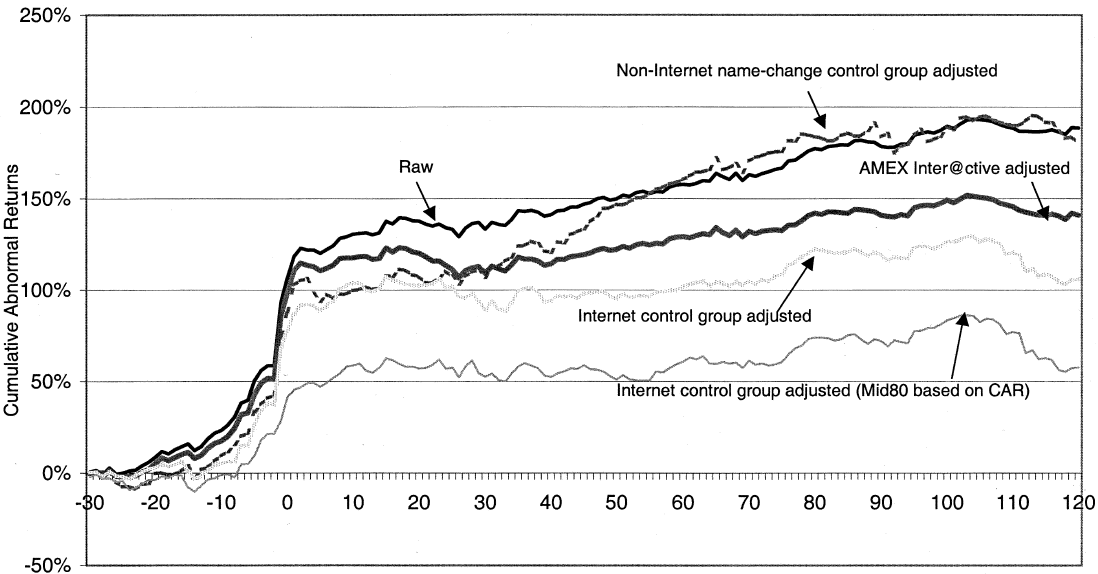
\includegraphics[width=\textwidth]{event_1}
\caption{Cumulative abnormal returns earned around the announcement date by firms changing their names to dotcom names}
\label{fig:cars}
\end{figure}

The CARs are also graphed in Figure \ref{fig:cars}. The dotcom effect is remarkably strong across all firms. The cumulative abnormal returns are positive and significant across event windows surrounding the announcement date, for firms announcing name changes between June 1998 and July 1999. For example, in Panel A of Table II, over the five-day period from day $-2$ to day $+2$, all firms earn a strongly statistically significant abnormal return of 53\%. Over the entire 61-day period from day $-30$ to day $+30$, all firms earn a significant 89\%, with a t-statistic of 6.2 (not reported in the table). We observe similar striking abnormal returns in all periods surrounding the announcement day.

$[\ldots]$

\newpage
\printbibliography

\end{document}
